\chapterimage{chapter_head_1.pdf} 
\chapter{El modo teselado}

Este capítulo explica el funcionamiento del modo teselado. La lista de ejercicios y el tiempo estimado (en minutos) para su realización se muestran en la Tabla \ref{c7_tab:ejercios}.

\begin{table}[t]
	\centering
	\caption{Ejercicios del capítulo y tiempo estimado para su realización.}
	\begin{tabular}{|c|c|}
		\hline 
		Ejercicio & Tiempo \\ 
		\hline 
		7.1 & 10' \\ 
		7.2 & 10' \\ 
		7.3 & 40' \\ 
		7.4 & 15' \\ 
		7.5 & 30' \\ 
		7.6 & 15' \\ 
		\hline 
	\end{tabular} 
	\label{c7_tab:ejercios}
\end{table}


% -----------------------------------------------------
% -----------------------------------------------------
% -----------------------------------------------------
% -----------------------------------------------------
\section{Introducción}
El modo teselado permite muchas más posibilidades a la hora de realizar videjuegos con gráficos que el modo framebuffer. 

% -----------------------------------------------------
% -----------------------------------------------------
\section{Funcionamiento básico del modo teselado}
En el modo teselado, la pantalla se divide en celdas conocidas como teselas. Una tesela es un bitmap de 8x8 que representa un gráfico que se quiere mostrar en una de las celdas en las que se divide la pantalla. 

Para definir una tesela, se deberá declarar un vector de 64 elementos ($8*8=64$) del tipo \textit{u8}. 

Por ejemplo, el siguiente código define las figuras del comecocos, del fantasma y un fondo:

\begin{lstlisting}
u8 comecocos[64] =
{
	2,2,1,1,1,1,2,2,
	2,2,1,1,1,1,1,2,
	2,2,2,1,1,1,1,1,
	2,2,2,2,1,1,1,1,
	2,2,2,2,1,1,1,1,
	2,2,2,1,1,1,1,1,
	2,2,1,1,1,1,1,2,
	2,2,1,1,1,1,2,2,
};

u8 fantasma[64] =
{
	2,2,2,3,3,2,2,2,
	2,3,3,3,3,3,3,2,
	3,3,3,3,3,3,3,3,
	3,4,2,3,3,4,2,3,
	3,4,2,3,3,4,2,3,
	3,3,3,3,3,3,3,3,
	3,3,3,3,3,3,3,3,
	3,2,3,2,2,3,2,3
};

u8 fondo[64] =
{
	2,2,2,2,2,2,2,2,
	2,2,2,2,2,2,2,2,
	2,2,2,2,2,2,2,2,
	2,2,2,2,2,2,2,2,
	2,2,2,2,2,2,2,2,
	2,2,2,2,2,2,2,2,
	2,2,2,2,2,2,2,2,
	2,2,2,2,2,2,2,2
};
\end{lstlisting}

Como se puede comprobar, se han definido los píxeles que componen la figura que representa la tesela. Se pueden definir hasta 1024 teselas diferentes. Existen dos formas de especificar los colores de los píxeles de las teselas:

\begin{itemize}
\item Modo de 256 colores: A cada píxel se le asigna un índice de la paleta de colores. El índice por lo tanto será un entero de 8 bits, con un valor comprendido entre 0 y 255. Este es el modo que se usará en esta sección. Por ejemplo, en las teselas anteriores, el número 1 indica el color almacenado en la posición 1 de la paleta de colores, el número 2 se refiere a la segunda posición, etc. 
%
\item Modo de 16 colores: En este caso un píxel es un índice a una paleta de 16 colores. Por lo tanto el índice será un entero de 4 bits, con un valor comprendido entre 0 y 15. Aunque este modo requiere menos memoria, dejando así más espacio para teselas y otros elementos en la VRAM, la calidad de la imagen renderizada se puede ver comprometida al disponer de solo 16 colores diferentes en cada tesela.
\end{itemize}

Para especificar los colores (en el modo de 256 colores), se debe modificar (en el programa principal) la paleta de colores mediante la variable \textit{BG\_PALETTE}. 

Por ejemplo, el código siguiente define los cuatro colores usados en las definiciones de las teselas anteriores:

\begin{lstlisting}
	BG_PALETTE[1]=RGB15(28,0,0);
	BG_PALETTE[2]=RGB15(0,20,0);
	BG_PALETTE[3]=RGB15(0,0,31);
	BG_PALETTE[4]=RGB15(31,31,31);
\end{lstlisting}
	
Como se puede comprobar, la posición 1 de la paleta se refiere a un color rojo, la 2 a uno verde, la 3 a uno azul y la 4 al color blanco.

En este modo de funcionamiento, el número de colores está limitado a 256 (de 0 a 255), número que se puede representar usando un byte. Por lo tanto, una tesela ocupa en memoria $8*8*1=64$ bytes. 

Para definir cómo se muestran las teselas en la pantalla se puede declarar un vector que tendrá tantos elementos como teselas queramos mostrar. Por ejemplo, si queremos mostrar toda la pantalla, será necesario declarar el vector con 768 elementos del tipo u16 ($32*24=768$). En dicho vector, comúnmente llamado mapa de teselas, se especifica la tesela a mostrar usando un número entero (de 2 bytes). El identificador de la tesela es el orden en el que estará almacenada en la memoria. 

El siguiente código declara el mapa de teselas para que cubra toda la pantalla (24 filas y 32 columnas):

\begin{lstlisting}
u16 mapData[768] =
{
1,2,2,2,2,2,2,2, 2,2,2,2,2,2,2,2,  2,2,2,2,2,2,2,2, 2,2,2,2,2,2,2,2,
2,2,2,3,2,2,2,2, 2,2,2,2,2,2,2,2,  2,2,2,2,2,2,2,2, 2,2,2,2,2,2,2,2,
2,3,2,2,2,2,2,2, 2,2,2,2,2,2,2,2,  2,2,2,2,2,2,2,2, 2,2,2,2,2,2,2,2,
2,2,2,2,2,2,2,2, 2,2,2,2,2,2,2,2,  2,2,2,2,2,2,2,2, 2,2,2,2,2,2,2,2,

2,2,2,2,2,2,2,2, 2,2,2,2,2,2,2,2,  2,2,2,2,2,2,2,2, 2,2,2,2,2,2,2,2,
2,2,2,2,2,2,2,2, 2,2,2,2,2,2,2,2,  2,2,2,2,2,2,2,2, 2,2,2,2,2,2,2,2,
2,2,2,2,2,2,2,2, 2,2,2,2,2,2,2,2,  2,2,2,2,2,2,2,2, 2,2,2,2,2,2,2,2,
2,2,2,2,2,2,2,2, 2,2,2,2,2,2,2,2,  2,2,2,2,2,2,2,2, 2,2,2,2,2,2,2,2,

2,2,2,2,2,2,2,2, 2,2,2,2,2,2,2,2,  2,2,2,2,2,2,2,2, 2,2,2,2,2,2,2,2,
2,2,2,2,2,2,2,2, 2,2,2,2,2,2,2,2,  2,2,2,2,2,2,2,2, 2,2,2,2,2,2,2,2,
2,2,2,2,2,2,2,2, 2,2,2,2,2,2,2,2,  2,2,2,2,2,2,2,2, 2,2,2,2,2,2,2,2,
2,2,2,2,2,2,2,2, 2,2,2,2,2,2,2,2,  2,2,2,2,2,2,2,2, 2,2,2,2,2,2,2,2,

2,2,2,2,2,2,2,2, 2,2,2,2,2,2,2,2,  2,2,2,2,2,2,2,2, 2,2,2,2,2,2,2,2,
2,2,2,2,2,2,2,2, 2,2,2,2,2,2,2,2,  2,2,2,2,2,2,2,2, 2,2,2,2,2,2,2,2,
2,2,2,2,2,2,2,2, 2,2,2,2,2,2,2,2,  2,2,2,2,2,2,2,2, 2,2,2,2,2,2,2,2,
2,2,2,2,2,2,2,2, 2,2,2,2,2,2,2,2,  2,2,2,2,2,2,2,2, 2,2,2,2,2,2,2,2,

2,2,2,2,2,2,2,2, 2,2,2,2,2,2,2,2,  2,2,2,2,2,2,2,2, 2,2,2,2,2,2,2,2,
2,2,2,2,2,2,2,2, 2,2,2,2,2,2,2,2,  2,2,2,2,2,2,2,2, 2,2,2,2,2,2,2,2,
2,2,2,2,2,2,2,2, 2,2,2,2,2,2,2,2,  2,2,2,2,2,2,2,2, 2,2,2,2,2,2,2,2,
2,2,2,2,2,2,2,2, 2,2,2,2,2,2,2,2,  2,2,2,2,2,2,2,2, 2,2,2,2,2,2,2,2,

2,2,2,2,2,2,2,2, 2,2,2,2,2,2,2,2,  2,2,2,2,2,2,2,2, 2,2,2,2,2,2,2,2,
2,2,2,2,2,2,2,2, 2,2,2,2,2,2,2,2,  2,2,2,2,2,2,2,2, 2,2,2,2,2,2,2,2,
2,2,2,2,2,2,2,2, 2,2,2,2,2,2,2,2,  2,2,2,2,2,2,2,2, 2,2,2,2,2,2,2,2,
2,2,2,2,2,2,2,2, 2,2,2,2,2,2,2,2,  2,2,2,2,2,2,2,2, 2,2,2,2,2,2,2,2
};
\end{lstlisting}

	
Como se puede comprobar, el elemento que se situará en la fila 0, columna 0 es la tesela con identificador 1 que será la que se almacenará en la memoria en primer lugar (será el comecocos), y la que se situará a su derecha es la tesela con identificador 2, que será la que se almacenará en segundo lugar (será el fondo). Además se mostrarán dos fantasmas, uno situado en la fila 1, columna 3, y el otro situado en la fila 2, columna 1. Las teselas que se muestran en cada posición se podrán modificar durante el transcurso del programa.

El mapa de teselas ocupará, en este caso, $768*2=1\ 536$ bytes. Este vector se copiará en la memoria del fondo para que el motor gráfico sepa qué teselas tiene que mostrar en la pantalla.

Una de las principales ventajas de este modo es el ahorro en el uso de memoria que proporciona esta forma de trabajar. Esto es debido a que el mapa de teselas especifica donde está almacenada la tesela a mostrar, no el contenido de la misma. Es decir, en vez de guardar $24*32*64 = 49\ 152$ bytes (24 filas, 32 columnas y cada tesela de $8\times8$ píxeles de 1 byte), se almacena $24*32*2 = 1\ 536$ bytes (24 filas, 32 columnas y 2 bytes por cada identificador de la tesela) más 64 bytes por cada tesela usada. Como en el ejemplo anterior se usaban tres teselas, el tamaño total de memoria que se necesita es $1\ 536 + 64*3 = 1\ 728$ bytes, lo que supone un ahorro de más del 95\% de memoria.

Con respecto al modo framebuffer el ahorro de memoria es incluso mayor. En el modo framebuffer especificamos el color de cada uno de los 192x256 píxeles usando un número de 2 bytes. Por lo tanto, se necesitan $192*256*2=98\ 302$ bytes. 

Para configurar el modo teselado, deberemos usar las siguientes instrucciones:

\begin{lstlisting}
	REG_POWERCNT = POWER_ALL_2D;
	REG_DISPCNT  = MODE_0_2D    | DISPLAY_BG0_ACTIVE ;
	VRAM_A_CR    = VRAM_ENABLE  | VRAM_A_MAIN_BG ;
	BGCTRL [0]   = BG_32x32     | BG_COLOR_256 | BG_MAP_BASE(0) | BG_TILE_BASE(1);
\end{lstlisting}

La línea 1 activa ambos motores gráficos. En la segunda línea indicamos que vamos a usar el modo 0 y el fondo 0 del motor principal (ver Figura \ref{fig_c5_modulos}). En la tercera línea activamos el banco de memoria \textit{VRAM\_A} y lo asignamos como memoria de fondos del motor principal. 

La cuarta línea se utiliza para configurar la memoria de fondos del fondo 0:
\begin{itemize}
	\item Con \textit{BG\_32\_32} elegimos el número de teselas máximo que podemos usar. Hay cuatro posibilidades $32\times32$, $32\times64$, $64\times32$ y $64\times64$. En nuestro caso se ha seleccionado $32\times32$.
	%
	\item Con \textit{BG\_COLOR\_256} indicamos que las teselas tendrán 256 colores que se especificarán en la paleta.
	%
	\item Con \textit{ BG\_MAP\_BASE(0)} indicamos donde se va a guardar el mapa de teselas. En este caso el mapa de teselas se almacenará en el primer bloque (para mapas) de la \textit{VRAM\_A}.
	%
	\item Por último, con \textit{BG\_TILE\_BASE(1)} indicamos donde se almacenarán las teselas, que en este caso es a partir del segundo bloque (para teselas) de la \textit{VRAM\_A}.
\end{itemize}
  

La memoria \textit{VRAM\_A} tiene un tamaño de 128KB (ver Tabla \ref{tab_c5_vram}). Tanto la memoria de teselas como las teselas se deben copiar a este banco de memoria. Los mapas de teselas se almacenan en bloques de 2KB. Hay 32 posibles posiciones (de la 0 a la 31). En este ejemplo, el mapa de teselas se almacenará en el primer bloque mediante la macro \textit{BG\_MAP\_BASE(0)}. Como el mapa de teselas ocupa $24*32*2 = 1\ 536$ bytes, cabe perfectamente en un único bloque de 2KB. Si no cupiera, se deberían usar más bloques.

Las teselas se guardan en bloques de 16KB. Hay 16 posibles posiciones (de la 0 a la 15). En este ejemplo, las tres teselas se almacenarán en el segundo bloque mediante la macro \textit{BG\_TILE\_BASE(1)}. Como las tres teselas ocupan $8*8*1*3 = 192$ bytes, cabe perfectamente en un único bloque de 16KB. Si no cupiera, se deberían usar más bloques. 

Hay que tener en cuenta que la zona usada para almacenar el mapa de teselas no se puede solapar con la zona usada para almacenar las teselas. Por eso las teselas empiezan en el bloque 1, puesto que parte de la memoria del bloque 0 ya está ocupada por el mapa de teselas.

Una vez configurado el modo teselado, hemos de copiar a memoria tanto el mapa de teselas como las propias teselas. El código siguiente muestra este proceso:

\begin{lstlisting}
	static u8*  tileMemory = (u8*)  BG_TILE_RAM(1);
	static u16* mapMemory  = (u16*) BG_MAP_RAM(0);

	// Copia de teselas
	dmaCopy(comecocos,tileMemory + 64,  sizeof(comecocos));
	dmaCopy(fondo,    tileMemory + 128, sizeof(fondo));
	dmaCopy(fantasma, tileMemory + 192, sizeof(fantasma));

	// Copia del mapa de teselas a la memoria gráfica
	pos_mapData = 0;
	for(i=0;i<32;i++)
		for(j=0;j<24;j++)
		{
			pos_mapMemory            = i*24+j;
			mapMemory[pos_mapMemory] = mapData[pos_mapData];
			pos_mapData ++;
		}
\end{lstlisting}

En las dos primeras líneas creamos dos variables para acceder a la zona de la memoria en VRAM\_A donde estará almacenado el mapa de teselas y a la zona de memoria (también en VRAM\_A) donde estarán almacenadas las teselas. Es importante destacar que ambas variables se refieren a posiciones de memoria dentro de la \textit{VRAM\_A}, aunque cada una apunta a una zona diferente dentro de esta memoria.

En las líneas 5, 6 y 7 se copian las teselas a la zona de memoria que le corresponde, empezando por \textit{tileMemory + 64} para la primera tesela. En este caso, la primera tesela es el comecocos, seguida del fondo y por último el fantasma. Por lo tanto, en el mapa de teselas pondremos 1 cuando queramos mostrar el comecocos, 2 para el fondo y 3 para el fantasma. Es importante destacar que las teselas se han empezado a almacenar a partir de la posición base + 64, puesto que la primera tesela que usamos tiene como índice 1 (y no 0). El desplazamiento es de 64 bytes puesto que cada tesela, en el modo de 256 colores, ocupa $8\times8$ píxeles de un byte, es decir 64 bytes. Si se especificara las teselas en el modo de 16 colores, el desplazamiento sería de 32 bytes, ya que en este caso la tesela ocupa $8\times8$ píxeles de un medio byte (4 bits).

En las líneas 11 a 17 se copia el mapa de teselas a la memoria gráfica.

\begin{example}
A continuación se muestra el código completo del programa (\textit{teselas1.c}) que muestra como resultado el gráfico que se muestra en la Figura \ref{fig_p2_c3_comecocos}

\begin{lstlisting}
#include <nds.h>
#include <stdio.h>

u8 comecocos[64] =
{
	2,2,1,1,1,1,2,2,
	2,1,1,1,1,1,2,2,
	1,1,1,1,1,2,2,2,
	1,1,1,1,2,2,2,2,
	1,1,1,1,2,2,2,2,
	1,1,1,1,1,2,2,2,
	2,1,1,1,1,1,2,2,
	2,2,1,1,1,1,2,2,
};

u8 fondo[64] =
{
	2,2,2,2,2,2,2,2,
	2,2,2,2,2,2,2,2,
	2,2,2,2,2,2,2,2,
	2,2,2,2,2,2,2,2,
	2,2,2,2,2,2,2,2,
	2,2,2,2,2,2,2,2,
	2,2,2,2,2,2,2,2,
	2,2,2,2,2,2,2,2
};

u8 fantasma[64] =
{
	2,2,2,3,3,2,2,2,
	2,3,3,3,3,3,3,2,
	3,3,3,3,3,3,3,3,
	3,4,2,3,3,4,2,3,
	3,4,2,3,3,4,2,3,
	3,3,3,3,3,3,3,3,
	3,3,3,3,3,3,3,3,
	3,2,3,2,2,3,2,3
};

u16 mapData[768] =
{
1,2,2,2,2,2,2,2, 2,2,2,2,2,2,2,2,  2,2,2,2,2,2,2,2, 2,2,2,2,2,2,2,2,
2,2,2,3,2,2,2,2, 2,2,2,2,2,2,2,2,  2,2,2,2,2,2,2,2, 2,2,2,2,2,2,2,2,
2,3,2,2,2,2,2,2, 2,2,2,2,2,2,2,2,  2,2,2,2,2,2,2,2, 2,2,2,2,2,2,2,2,
2,2,2,2,2,2,2,2, 2,2,2,2,2,2,2,2,  2,2,2,2,2,2,2,2, 2,2,2,2,2,2,2,2,

2,2,2,2,2,2,2,2, 2,2,2,2,2,2,2,2,  2,2,2,2,2,2,2,2, 2,2,2,2,2,2,2,2,
2,2,2,2,2,2,2,2, 2,2,2,2,2,2,2,2,  2,2,2,2,2,2,2,2, 2,2,2,2,2,2,2,2,
2,2,2,2,2,2,2,2, 2,2,2,2,2,2,2,2,  2,2,2,2,2,2,2,2, 2,2,2,2,2,2,2,2,
2,2,2,2,2,2,2,2, 2,2,2,2,2,2,2,2,  2,2,2,2,2,2,2,2, 2,2,2,2,2,2,2,2,

2,2,2,2,2,2,2,2, 2,2,2,2,2,2,2,2,  2,2,2,2,2,2,2,2, 2,2,2,2,2,2,2,2,
2,2,2,2,2,2,2,2, 2,2,2,2,2,2,2,2,  2,2,2,2,2,2,2,2, 2,2,2,2,2,2,2,2,
2,2,2,2,2,2,2,2, 2,2,2,2,2,2,2,2,  2,2,2,2,2,2,2,2, 2,2,2,2,2,2,2,2,
2,2,2,2,2,2,2,2, 2,2,2,2,2,2,2,2,  2,2,2,2,2,2,2,2, 2,2,2,2,2,2,2,2,

2,2,2,2,2,2,2,2, 2,2,2,2,2,2,2,2,  2,2,2,2,2,2,2,2, 2,2,2,2,2,2,2,2,
2,2,2,2,2,2,2,2, 2,2,2,2,2,2,2,2,  2,2,2,2,2,2,2,2, 2,2,2,2,2,2,2,2,
2,2,2,2,2,2,2,2, 2,2,2,2,2,2,2,2,  2,2,2,2,2,2,2,2, 2,2,2,2,2,2,2,2,
2,2,2,2,2,2,2,2, 2,2,2,2,2,2,2,2,  2,2,2,2,2,2,2,2, 2,2,2,2,2,2,2,2,

2,2,2,2,2,2,2,2, 2,2,2,2,2,2,2,2,  2,2,2,2,2,2,2,2, 2,2,2,2,2,2,2,2,
2,2,2,2,2,2,2,2, 2,2,2,2,2,2,2,2,  2,2,2,2,2,2,2,2, 2,2,2,2,2,2,2,2,
2,2,2,2,2,2,2,2, 2,2,2,2,2,2,2,2,  2,2,2,2,2,2,2,2, 2,2,2,2,2,2,2,2,
2,2,2,2,2,2,2,2, 2,2,2,2,2,2,2,2,  2,2,2,2,2,2,2,2, 2,2,2,2,2,2,2,2,

2,2,2,2,2,2,2,2, 2,2,2,2,2,2,2,2,  2,2,2,2,2,2,2,2, 2,2,2,2,2,2,2,2,
2,2,2,2,2,2,2,2, 2,2,2,2,2,2,2,2,  2,2,2,2,2,2,2,2, 2,2,2,2,2,2,2,2,
2,2,2,2,2,2,2,2, 2,2,2,2,2,2,2,2,  2,2,2,2,2,2,2,2, 2,2,2,2,2,2,2,2,
2,2,2,2,2,2,2,2, 2,2,2,2,2,2,2,2,  2,2,2,2,2,2,2,2, 2,2,2,2,2,2,2,2
};

int main(void)
{
	int fila,columna,pos_mapMemory,pos_mapData;

	REG_POWERCNT = POWER_ALL_2D;
	REG_DISPCNT  = MODE_0_2D   | DISPLAY_BG0_ACTIVE ;
	VRAM_A_CR    = VRAM_ENABLE | VRAM_A_MAIN_BG ;
	BGCTRL[0]    = BG_32x32    | BG_COLOR_256 | BG_MAP_BASE(0) | BG_TILE_BASE(1);

	BG_PALETTE[1]=RGB15(28,0,0);
	BG_PALETTE[2]=RGB15(0,20,0);
	BG_PALETTE[3]=RGB15(0,0,31);
	BG_PALETTE[4]=RGB15(31,31,31);

	static u8*  tileMemory = (u8*)  BG_TILE_RAM(1);
	static u16*  mapMemory = (u16*) BG_MAP_RAM(0);

	dmaCopy(comecocos, tileMemory + 64,  sizeof(comecocos));
	dmaCopy(fondo,     tileMemory + 128, sizeof(fondo));
	dmaCopy(fantasma,  tileMemory + 192, sizeof(fantasma));

	pos_mapData = 0;
	for(fila=0;fila<24;fila++)
	  for(columna=0;columna<32;columna++)
	  {
        pos_mapMemory            = fila*32+columna;
        mapMemory[pos_mapMemory] = mapData[pos_mapData];
        pos_mapData ++;
	  }

	while(1)
	{
		swiWaitForVBlank();
	}
}
\end{lstlisting}
\end{example}

\begin{figure}[t]
	\centering
	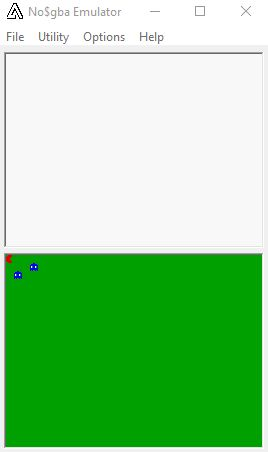
\includegraphics[height=9cm]{Figuras/C7/c7_teselas.jpg}
	\caption{Salida del programa de esta sección en la NDS}
	\label{fig_p2_c3_comecocos}
\end{figure}


\begin{exercise}
	Crea un proyecto con el código del ejemplo anterior y comprueba que funciona correctamente.
\end{exercise}

\begin{exercise}
A partir del ejercicio anterior, modifica el mapa de teselas para mostrar 5 comecocos y 10 fantasmas repartidos por la pantalla.
\end{exercise}
	

El programa anterior también se podría haber realizado sin tener que haber creado el mapa de teselas inicial. Para ello escribimos directamente el número de tesela en la posición de memoria que nos interese.
	
\begin{example}	
El siguiente programa (\textit{teselas2.c}) muestra un ejemplo:

\begin{lstlisting}
#include <nds.h>
#include <stdio.h>

u8 comecocos[64] =
{
2,2,1,1,1,1,2,2,
2,1,1,1,1,1,2,2,
1,1,1,1,1,2,2,2,
1,1,1,1,2,2,2,2,
1,1,1,1,2,2,2,2,
1,1,1,1,1,2,2,2,
2,1,1,1,1,1,2,2,
2,2,1,1,1,1,2,2,
};

u8 fondo[64] =
{
2,2,2,2,2,2,2,2,
2,2,2,2,2,2,2,2,
2,2,2,2,2,2,2,2,
2,2,2,2,2,2,2,2,
2,2,2,2,2,2,2,2,
2,2,2,2,2,2,2,2,
2,2,2,2,2,2,2,2,
2,2,2,2,2,2,2,2
};

u8 fantasma[64] =
{
2,2,2,3,3,2,2,2,
2,3,3,3,3,3,3,2,
3,3,3,3,3,3,3,3,
3,4,2,3,3,4,2,3,
3,4,2,3,3,4,2,3,
3,3,3,3,3,3,3,3,
3,3,3,3,3,3,3,3,
3,2,3,2,2,3,2,3
};

int main(void)
{
	int i, fila, columna;

	REG_POWERCNT = POWER_ALL_2D;
	REG_DISPCNT  = MODE_0_2D   | DISPLAY_BG0_ACTIVE ;
	VRAM_A_CR    = VRAM_ENABLE | VRAM_A_MAIN_BG ;
	BGCTRL[0]    = BG_32x32    | BG_COLOR_256 | BG_MAP_BASE(0) | BG_TILE_BASE(1);

	BG_PALETTE[1]=RGB15(28,0,0);
	BG_PALETTE[2]=RGB15(0,20,0);
	BG_PALETTE[3]=RGB15(0,0,31);
	BG_PALETTE[4]=RGB15(31,31,31);

	static u8*  tileMemory = (u8*)  BG_TILE_RAM(1);
	static u16*  mapMemory = (u16*) BG_MAP_RAM(0);

	dmaCopy(comecocos, tileMemory + 64,  sizeof(comecocos));
	dmaCopy(fondo,     tileMemory + 128, sizeof(fondo));
	dmaCopy(fantasma,  tileMemory + 192, sizeof(fantasma));

	// fondo
	for(i=0;i<32*24;i++)
		mapMemory[i] = 2;

	// comecocos en la fila 0, columna 0
	fila = 0; columna = 0;
	mapMemory[fila*32+columna] = 1;

	// fantasma en la fila 1, columna 3
	fila = 1; columna = 3;
	mapMemory[fila*32+columna] = 3;

	// fantasma en la fila 2, columna 1
	fila = 2; columna = 1;
	mapMemory[fila*32+columna] = 3;

	while(1)
	{
		swiWaitForVBlank();
	}
}
\end{lstlisting}
\end{example}		
	
Si queremos que la pantalla se modifique como respuesta a un evento, únicamente tenemos que cambiar la memoria de teselas (\textit{mapMemory}) correspondiente a la posición que queremos cambiar, modificando el índice a la tesela que queremos mostrar.

\begin{example}
Por ejemplo, el siguiente fragmento de código (el programa completo es \textit{teselas3.c}) mostrará al pulsar la tecla A de la NDS, un segundo comecocos en la celda situada en la fila 15 y columna 16:

\begin{lstlisting}
...
while(1)
{
	scanKeys();
	int key = keysDown();

	if (key & KEY_A)
	{
		fila                     = 15;
		columna                  = 16;
		pos_mapMemory            = fila*32+columna;
		mapMemory[pos_mapMemory] = 1;
	}
	swiWaitForVBlank();
}
\end{lstlisting}
\end{example}

\begin{exercise}
	Realiza un programa que mueva el comecocos por la pantalla usando para ello los botones de las flechas de la NDS. Debes tener en cuenta los límites de la pantalla.
\end{exercise}
	
	
% ------------------------------------------------------------------------
% ------------------------------------------------------------------------
% ------------------------------------------------------------------------
% ------------------------------------------------------------------------
\section{Funcionamiento avanzado del modo teselado}
El motor gráfico renderiza los fondos teselados a partir de las entradas del \textit{mapa} y la \textit{colección de teselas} a las que hace referencia, estando estos datos contenidos en la memoria de fondos de la VRAM. Teniendo en cuenta que cada motor gráfico puede gestionar un máximo de cuatro fondos, es necesario que cada fondo activado configure la localización de sus datos de mapas y teselas. Para ello se utiliza el registro de configuración del fondo, \textit{REG\_BGnCNT} o \textit{BGCTRL[n]}, donde \textit{n} hace referencia al índice del fondo, tomando valores de 0 a 3. Este registro reserva 4 bits para especificar el desplazamiento de las teselas (en múltiplos de 16 KB) y 5 bits para el mapa (en múltiplos de 2 KB), de tal forma que las teselas admiten $2^4 = 16$ posibles valores del desplazamiento base y los mapas admiten $2^5 = 32$. La Figura \ref{fig_p2_c3_reg_teselado} muestra el significado de cada uno de sus bits.

\begin{figure}[t]
\centering
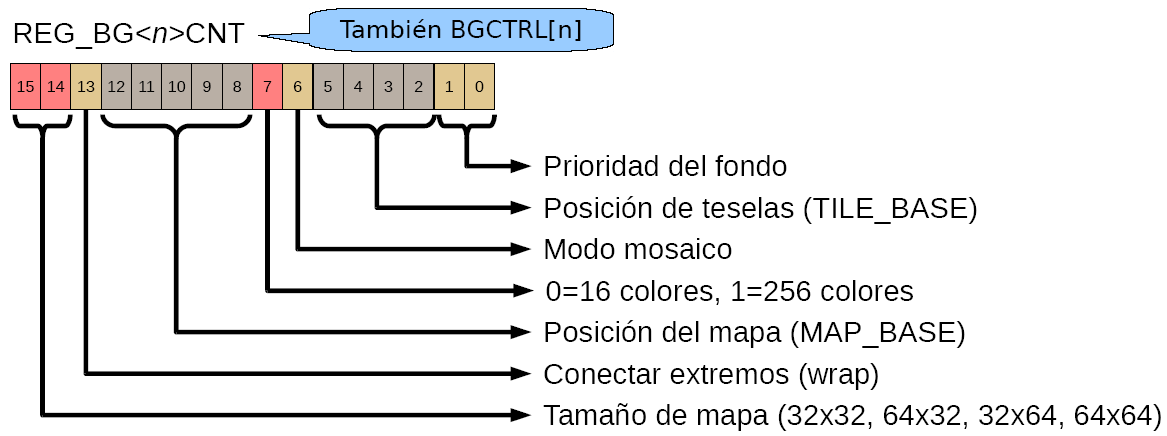
\includegraphics[height=4cm]{Figuras/C7/c7_reg_teselado.PNG}
\caption{Significados de los bits del registro \textit{REG\_BGnCNT}.}
\label{fig_p2_c3_reg_teselado}
\end{figure}

% ------------------------------------------------------------------------
% ------------------------------------------------------------------------
\subsection{Guardar mapas de teselas en la VRAM}
Un \textit{mapa de teselas} puede empezar en cualquier dirección múltiplo de 2KB entre 0 x 2KB y 31 x 2KB. Estos valores expresados en hexadecimal serían desde 0 x 0x800 hasta 31 x 0x800. Para que se facilite la configuración de las direcciones base, \textit{libnds} incluye la macro \textit{BG\_MAP\_BASE(n)}, donde \textit{n} se corresponde con el múltiplo de \textit{2KB} seleccionado, entre 0 y 31. Por ejemplo, si se indica en el registro de configuración del fondo que los datos del mapa se encuentran ubicados a partir de \textit{BG\_MAP\_BASE(1)}, significa que comenzarán en la posición de memoria \textit{0x0800} a partir del principio de la memoria de fondos. Análogamente, decir que lo hacen en \textit{BG\_MAP\_BASE(31)} significa que empiezan en la posición \textit{\textit{0xf800}}, tal y como se puede comprobar en la Figura \ref{fig_p2_c3_teselas3}.

\begin{figure}[t]
\centering
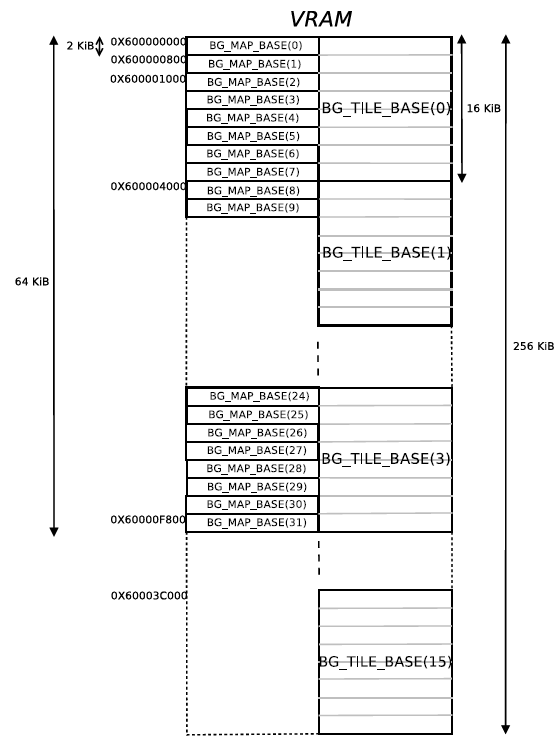
\includegraphics[height=14cm]{Figuras/C7/c7_mem_teselas.PNG}
\caption{Desplazamientos en la VRAM.}
\label{fig_p2_c3_teselas3}
\end{figure}

El motor de vídeo no tiene memoria física dedicada, por tanto, \textit{parte de la memoria VRAM se debe configurar para ser utilizada como memoria de fondos}. El motor gráfico principal utiliza como memoria de fondos el rango de memoria de \textit{0x06000000} a \textit{0x0607ffff} (512KB máximo) mientras que el secundario emplea el rango de \textit{0x06200000} a \textit{0x0621ffff} (128KB máximo). Todos los desplazamientos base de mapas y teselas se llevan a cabo tomando como dirección base el comienzo de estos rangos de memoria.

El tamaño de un mapa de teselas depende del tamaño del fondo:
\begin{itemize}
\item  Un mapa de $32\times32$ teselas será una sucesión de $32\times32$ entradas de 16 bits, por lo que el tamaño total será de $2\times32\times32 = 2KB$. Es decir, en este caso el mapa entero cabe antes de la siguiente dirección base de otro mapa.
%
\item  Sin embargo, para un fondo de $64\times64$ teselas, los datos del mapa requieren $2\times64\times64 = 8KB$, es decir, son necesarios cuatro bloques completos de $8KB$.
\end{itemize}

Estos cálculos se muestran de manera gráfica en la Figura \ref{fig_p2_c3_teselas2b}.

\begin{figure}[t]
\centering
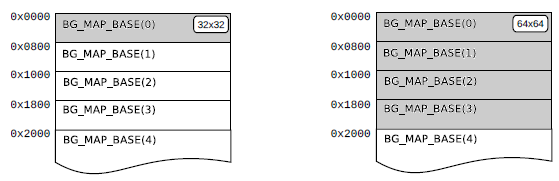
\includegraphics[height=4cm]{Figuras/C7/c7_mem_teselas2.PNG}
\caption{Cálculo del tamaño de un mapa de teselas.}
\label{fig_p2_c3_teselas2b}
\end{figure}

Como se ha comentado previamente cada una de las entradas del mapa se representa mediante un conjunto de 16 bits, donde los 10 bits menos significativos especifican la tesela, razón por la que el conjunto máximo de teselas es de  1024, las máximas referenciables con 10 bits. Los dos bits siguientes se utilizan para especificar el efecto de espejo en la tesela, es decir, si tiene una reflexión horizontal, vertical o ambas. Finalmente, para teselas que utilizan paletas de 16 colores, se utilizan los 4 bits más significativos para identificar la paleta de colores utilizada por esa tesela. La Figura \ref{fig_p2_c3_entmapateselas} muestra dicha distribución.

\begin{figure}[t]
\centering
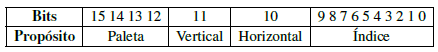
\includegraphics[height=1cm]{Figuras/C7/c7_bits_teselas.PNG}
\caption{Entradas del mapa de teselas.}
\label{fig_p2_c3_entmapateselas}
\end{figure}

\subsection{Guardar teselas en la VRAM}
En cuanto a las teselas, ocurre lo mismo que para los mapas, ya que ambos comparten la misma memoria de fondos y al igual que los mapas, utilizarán los desplazamientos para gestionar esa memoria como si estuviera organizada en bloques, sólo que en este caso, de \textit{tamaño 16KB}. La macro utilizada para especificar la dirección base es \textit{BG\_TILE\_BASE(n)}, donde \textit{n} toma valores entre 0 y 15. El número hace referencia al múltiplo de 16KB correspondiente, empezando en $0x0000$, desplazándose en múltiplos de $0x4000$ hasta el valor $0x3C000$, tal y como se puede observar en la Figura \ref{fig_p2_c3_teselas3}. 

% -----------------------------------------------------
% -----------------------------------------------------
% -----------------------------------------------------
% -----------------------------------------------------
\section{Mostrar más de un fondo a la vez}

% -----------------------------------------------------
% -----------------------------------------------------
\subsection{Ambos motores a la vez}
Para configurar el motor secundario se usarán instrucciones muy similares a las usadas para el motor principal. La principal diferencia es el uso del sufijo \textit{SUB} o la sustitución de \textit{MAIN} por \textit{SUB}.

\begin{example}
El siguiente programa (\textit{dosmotores.c}) muestra una composición de teselas en cada pantalla, la pantalla inferior usará el motor principal y la superior el secundario:
\begin{lstlisting}
#include <nds.h>
#include <stdio.h>

u8 verde[64] =
{
1,1,1,1,1,1,1,1,
1,1,1,1,1,1,1,1,
1,1,1,1,1,1,1,1,
1,1,1,1,1,1,1,1,
1,1,1,1,1,1,1,1,
1,1,1,1,1,1,1,1,
1,1,1,1,1,1,1,1,
1,1,1,1,1,1,1,1,
};

u8 rojo[64] =
{
2,2,2,2,2,2,2,2,
2,2,2,2,2,2,2,2,
2,2,2,2,2,2,2,2,
2,2,2,2,2,2,2,2,
2,2,2,2,2,2,2,2,
2,2,2,2,2,2,2,2,
2,2,2,2,2,2,2,2,
2,2,2,2,2,2,2,2,
};

int main( void )
{
  REG_POWERCNT    = POWER_ALL_2D;
  REG_DISPCNT     = MODE_0_2D | DISPLAY_BG0_ACTIVE;
  REG_DISPCNT_SUB = MODE_0_2D | DISPLAY_BG0_ACTIVE;
  VRAM_A_CR       = VRAM_ENABLE | VRAM_A_MAIN_BG;
  VRAM_C_CR       = VRAM_ENABLE | VRAM_C_SUB_BG;
  BGCTRL[0]    = BG_32x32| BG_COLOR_256 | BG_MAP_BASE(0) | BG_TILE_BASE(1);
  BGCTRL_SUB[0]= BG_32x32| BG_COLOR_256 | BG_MAP_BASE(0) | BG_TILE_BASE(1);

  static u8*  tileMemory    = (u8*)  BG_TILE_RAM(1);
  static u16* mapMemory     = (u16*) BG_MAP_RAM(0);
  static u8*  tileMemorySub = (u8*)  BG_TILE_RAM_SUB(1);
  static u16* mapMemorySub  = (u16*) BG_MAP_RAM_SUB(0);

  BG_PALETTE[1]     = RGB15(0,20,0);
  BG_PALETTE[2]     = RGB15(20,0,0);
  BG_PALETTE_SUB[1] = RGB15(0,20,0);
  BG_PALETTE_SUB[2] = RGB15(20,0,0);

  dmaCopy(verde, tileMemory + 64,     sizeof(verde));
  dmaCopy(rojo,  tileMemorySub + 64, sizeof(rojo));

  int fila,columna;

  for(fila=0;fila<24;fila++)
    for(columna=0;columna<32;columna++)
    {
      mapMemory   [fila*32+columna] = 1;  
      mapMemorySub[fila*32+columna] = 1;   
    }
	
  while(1)
  {
    swiWaitForVBlank();
  }
}
\end{lstlisting}
\end{example}

Como se puede comprobar, se configura el fondo 0 de cada uno de los motores para tener un mapa de teselas de $32\times32$ teselas. El motor principal almacenará el mapa de teselas y las teselas en la VRAM\_A. El motor secundario lo hará en la VRAM\_C. Hay que fijarse que aunque las macros usadas para indicar en que parte de la memoria se van a almacenar el mapa de teselas y las teselas son iguales, en realidad no se refieren a las mismas posiciones de memoria, pues cada fondo usa una memoria VRAM diferente.

Cada fondo almacena unicamente la tesela que va usar (líneas 48 y 49). Así para el fondo 0, la tesela en la posición 1 es la tesela \textit{verde}. Sin embargo, para el fondo 1, en la posición 1 se encontrará la tesela \textit{rojo}. 

Para ambos fondos, se rellena la pantalla completa con la tesela situada en primer lugar. El resultado final se muestra en la Figura \ref{c7_fig:dosmotores}.


\begin{figure}[t]
	\centering
	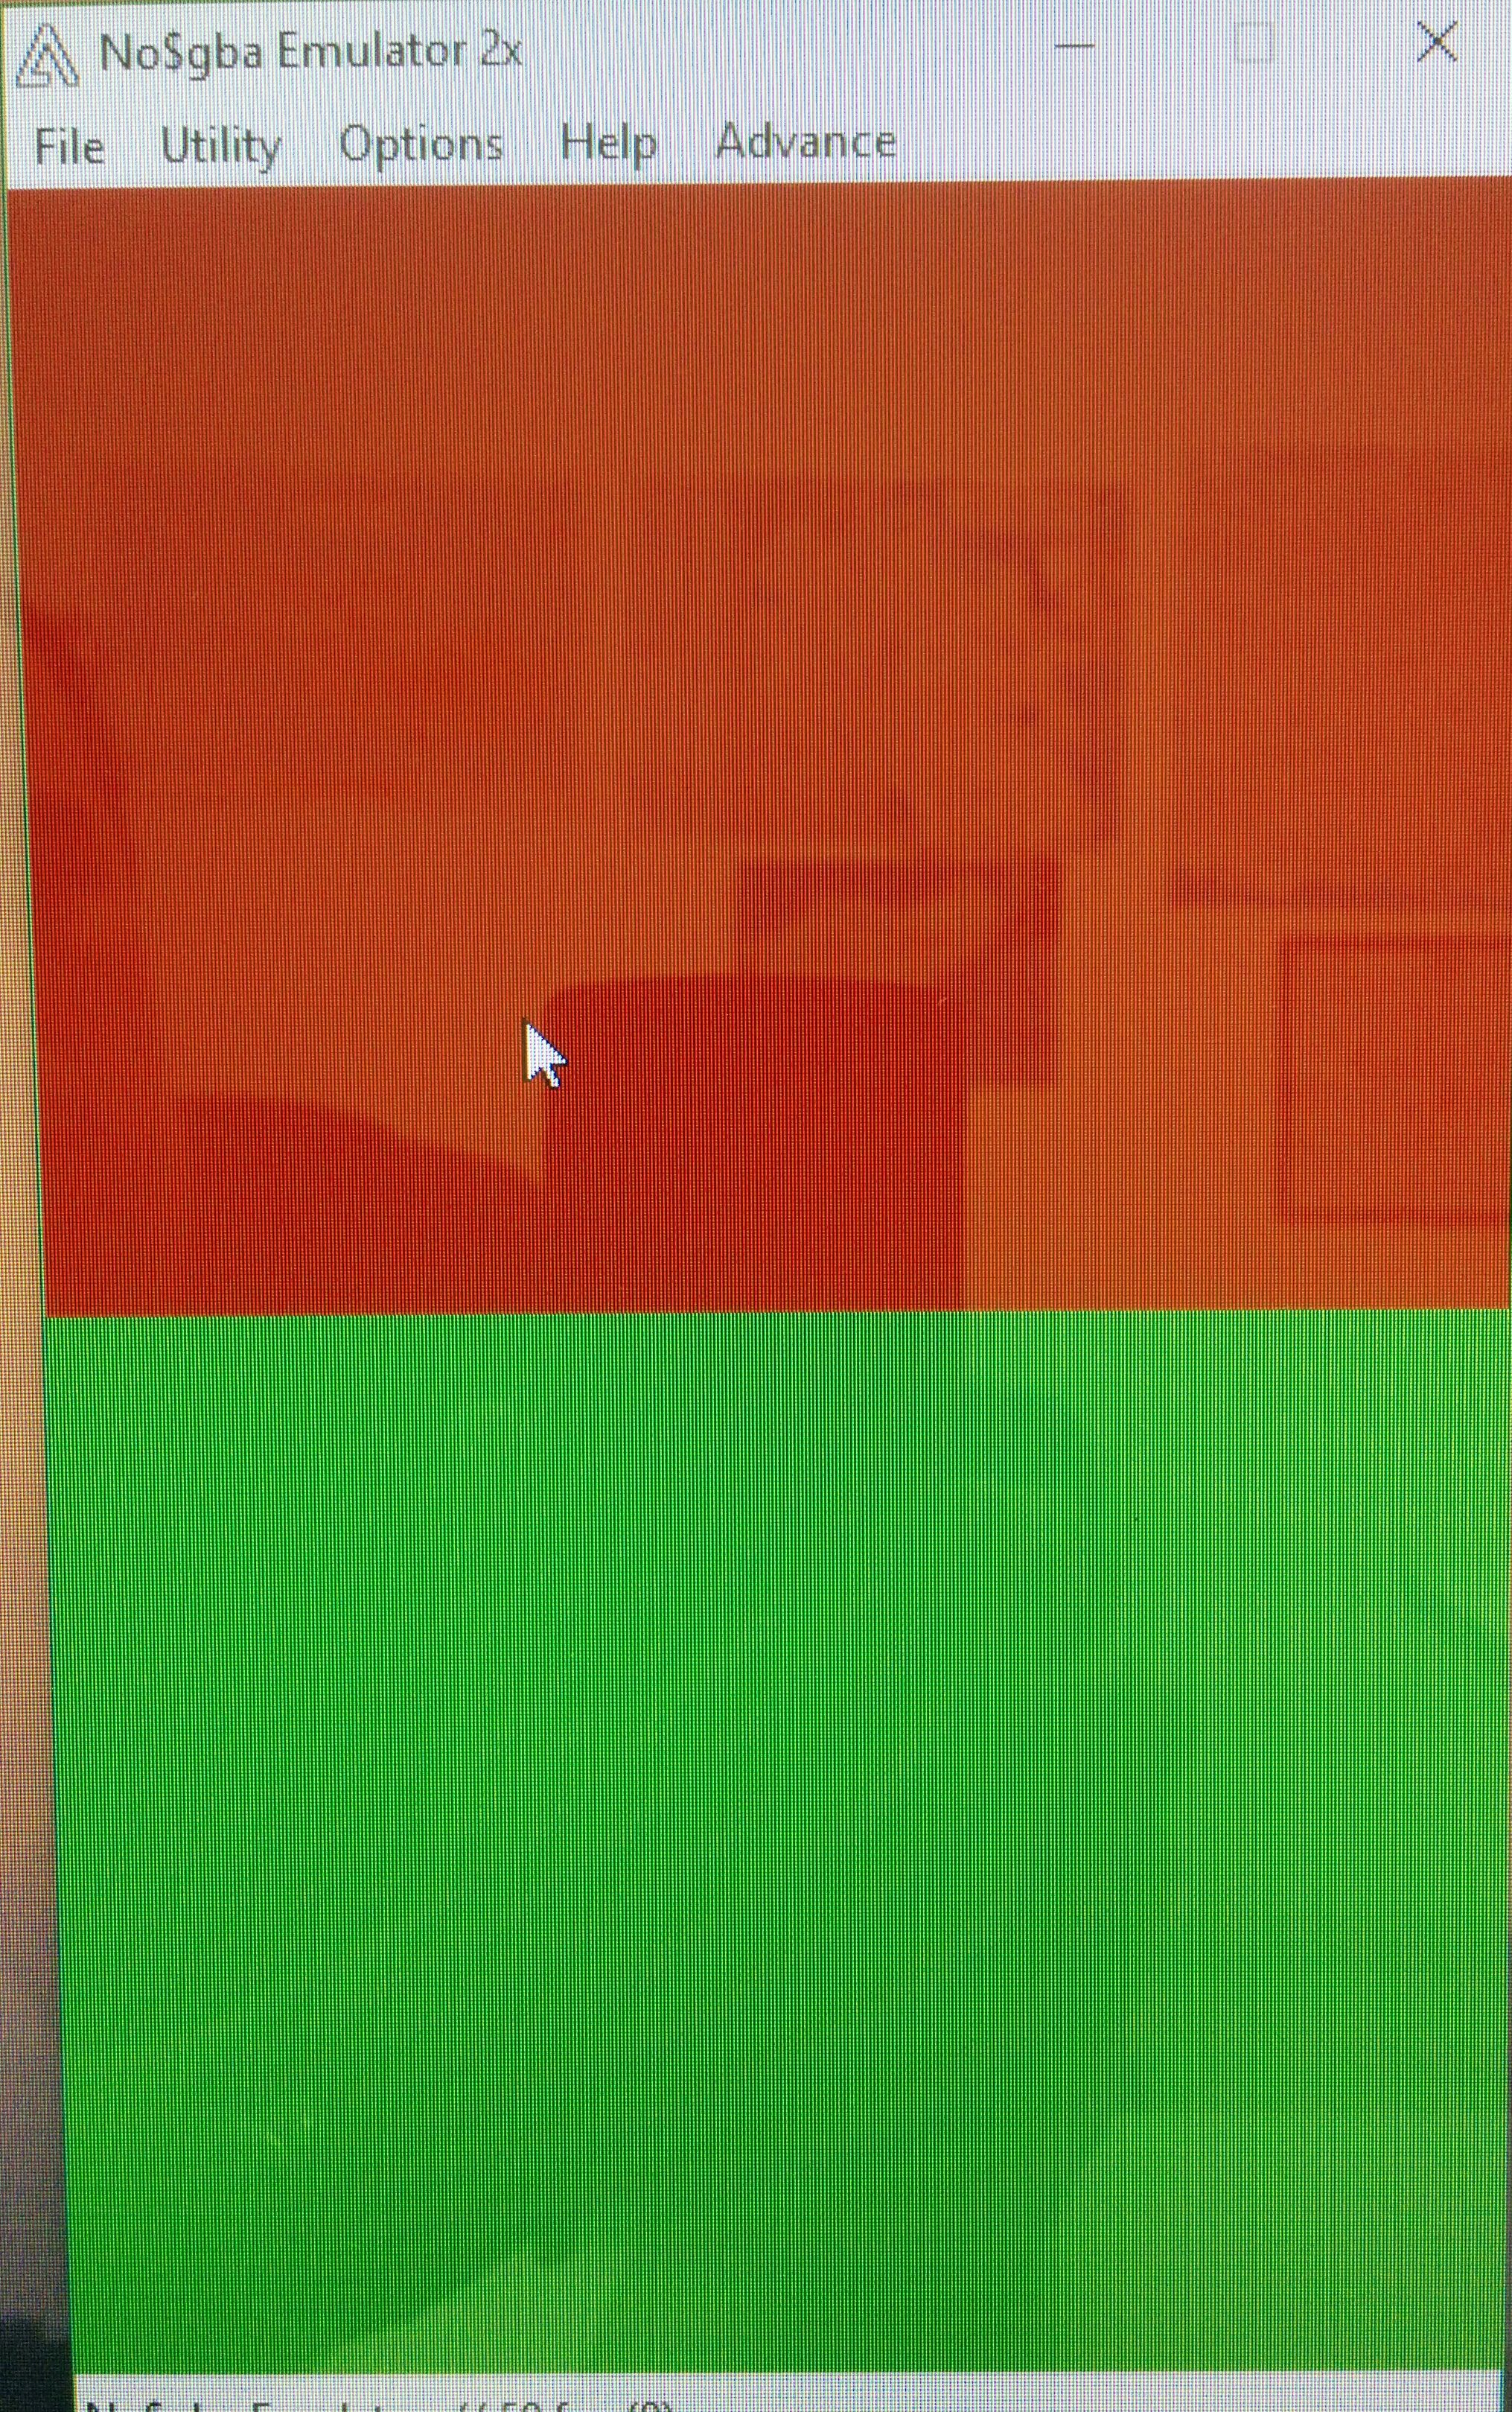
\includegraphics[height=6cm]{Figuras/C7/c7_dosmotores.jpg}
	\caption{Resultado del programa \textit{dosmotores.c}}
	\label{c7_fig:dosmotores}
\end{figure}


\begin{exercise}
Partiendo del programa anterior realiza las modificaciones que sean necesarias para que al pulsar la tecla \textit{A} de la NDS, se intercambien los colores mostrados en las pantallas. Al pulsar la tecla \textit{X} se volverá a la situación inicial.
\end{exercise}
% -----------------------------------------------------
% -----------------------------------------------------
\subsection{Superponer fondos en la misma pantalla}

\begin{example}
El siguiente programa (\textit{dosfondos.c}) muestra como superponer dos fondos en la misma pantalla:
\begin{lstlisting}
#include <nds.h>
#include <stdio.h>

u8 verde[64] =
{
1,1,1,1,1,1,1,1,
1,1,1,1,1,1,1,1,
1,1,1,1,1,1,1,1,
1,1,1,1,1,1,1,1,
1,1,1,1,1,1,1,1,
1,1,1,1,1,1,1,1,
1,1,1,1,1,1,1,1,
1,1,1,1,1,1,1,1,
};

u8 rojo[64] =
{
2,2,2,2,2,2,2,2,
2,2,2,2,2,2,2,2,
2,2,2,2,2,2,2,2,
2,2,2,2,2,2,2,2,
2,2,2,2,2,2,2,2,
2,2,2,2,2,2,2,2,
2,2,2,2,2,2,2,2,
2,2,2,2,2,2,2,2,
};

int main( void )
{
  REG_POWERCNT = POWER_ALL_2D;
  REG_DISPCNT  = MODE_0_2D | DISPLAY_BG0_ACTIVE | DISPLAY_BG1_ACTIVE;
  VRAM_A_CR    = VRAM_ENABLE | VRAM_A_MAIN_BG;
  BGCTRL[0]    = BG_32x32 | BG_COLOR_256 | 
                 BG_MAP_BASE(0) | BG_TILE_BASE(1) | BG_PRIORITY(1);  
  BGCTRL[1]    = BG_32x32 | BG_COLOR_256 | 
                 BG_MAP_BASE(1) | BG_TILE_BASE(2) | BG_PRIORITY(0);  
	
  static u8*  tileMemoryB0  = (u8*)  BG_TILE_RAM(1);
  static u8*  tileMemoryB1  = (u8*)  BG_TILE_RAM(2);
  
  static u16* mapMemoryB0   = (u16*) BG_MAP_RAM(0);
  static u16* mapMemoryB1   = (u16*) BG_MAP_RAM(1);
	
  BG_PALETTE[1] = RGB15(0,20,0);
  BG_PALETTE[2] = RGB15(20,0,0);
	
  dmaCopy(verde, tileMemoryB0 + 64,  sizeof(verde));
  dmaCopy(rojo,  tileMemoryB1 + 64, sizeof(rojo));
	
  int fila, columna;
	
  for(fila=0;fila<24;fila++)
    for(columna=0;columna<32;columna++)
    {
	  mapMemoryB0[fila*32+columna] = 1;     
	  if (columna>16)
	    mapMemoryB1[fila*32+columna] = 1;   
    }
	
  while(1)
  {
    swiWaitForVBlank();
  }
}
\end{lstlisting}
\end{example}

Tal como muestra el código, se han configurado dos fondos para el motor principal. El primero de ellos (fondo 0) estará abajo por tener menos prioridad. El segundo (fondo 1) se mostrará por encima del fondo anterior. La prioridad se establece con la macro \textit{BG\_PRIORITY(N)}, donde \textit{N} es la prioridad y admite valores de 0 a 3. Número más bajos de \textit{N} indican más prioridad (más arriba en el orden de visualización). Ambos fondos se almacenarán en la VRAM\_A, situando los mapas de teselas y las teselas en zonas no coincidentes. El primer fondo se pinta completamente con la tesela de color verde. El segundo fondo pinta únicamente las columnas de la derecha con las tesela de color rojo, permitiendo que en la parte izquierda se vea el primer fondo.
El resultado final se muestra en la Figura \ref{c7_fig:dosfondos}.


\begin{figure}[t]
	\centering
	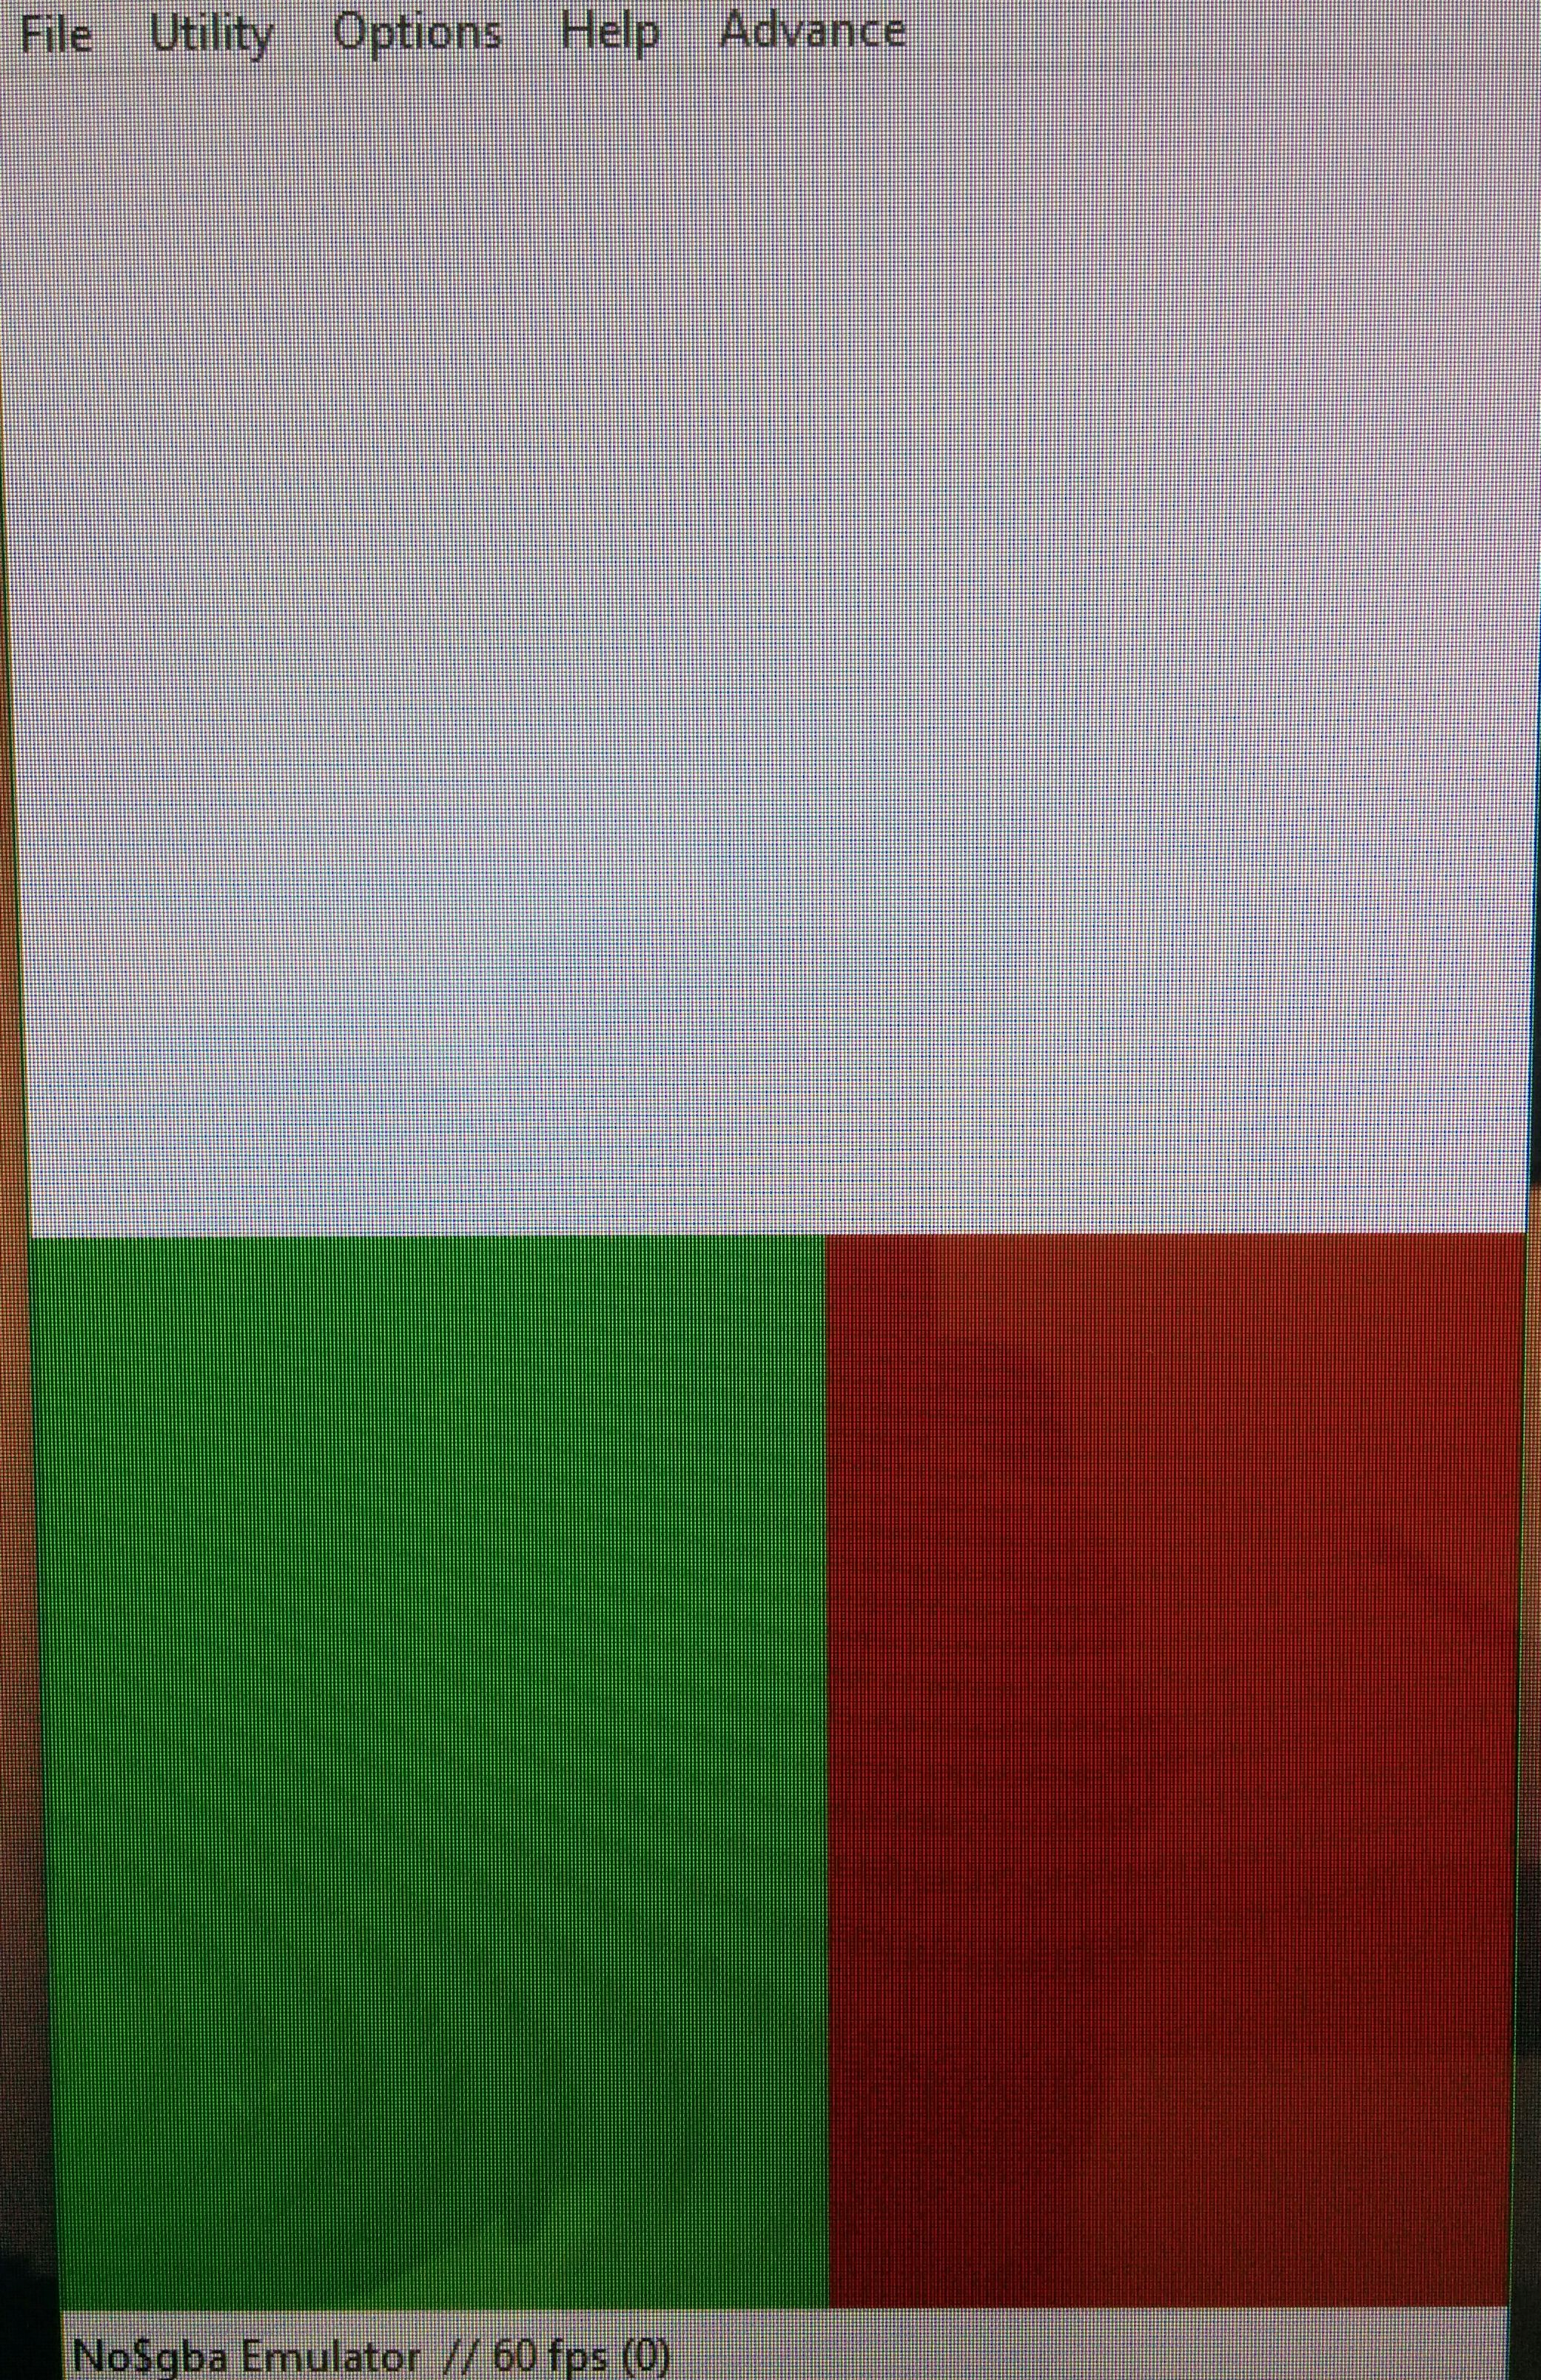
\includegraphics[height=6cm]{Figuras/C7/c7_dosfondos.jpg}
	\caption{Resultado del programa \textit{dosfondos.c}}
	\label{c7_fig:dosfondos}
\end{figure}


\begin{exercise}
	Realiza un programa que muestre en la pantalla inferior cuatro fondos diferentes. De más profundo a mas exterior los colores de cada uno de los fondos serán verde, rojo, azul y amarillo. Deberás pintar las teselas de forma que se vea claro el orden de los fondos.
\end{exercise}

% -----------------------------------------------------
% -----------------------------------------------------
\section{Ejercicios avanzados}
\begin{exercise}
	Realiza un programa que muestre en cada pantalla cuatro fondos diferentes.
\end{exercise}
	